%! Author = charon
%! Date = 1/9/24

\documentclass{beamer}

\usetheme{metropolis}

\usepackage{multicol}
\usepackage{graphicx}
\usepackage{listings}
\usepackage{biblatex}
\usepackage{tikz}
\usepackage{csquotes}
\usepackage{glossaries}
\usetikzlibrary{shapes.geometric, arrows}

\title{Fuzzing}
\subtitle{Eine Einführung in die Welt des Fuzzings}
\date{13.12.2024}
\author{Sebastian Peschke}
\institute{Hochschule für angewandte Wissenschaften Hof}

\addbibresource{src.bib}
\begin{document}
    \maketitle
    %! Author = charon
%! Date = 12/9/24

\section{Einführung}\label{sec:einfuhrung}
\begin{frame}{Was ist Fuzzing?}
    \blockquote{\enquote{Fuzzing is a vulnerability discovery solution that resonates with random-mutation, feedback-driven,
        coverage-guided, constraint-guided, seed-scheduling, and target-oriented strategies.
        Each technique is wrapped beneath the black-, white-, and grey-box fuzzers to uncover diverse vulnerabilities.}Sanoop et al.~\cite{fuzzing_methods}}
\end{frame}
\begin{frame}{Was ist Fuzzing?}
    \blockquote{\enquote{Fuzzing is a \alert{vulnerability discovery solution} that resonates with random-mutation, feedback-driven,
        coverage-guided, constraint-guided, seed-scheduling, and target-oriented \alert{strategies}.
        Each \alert{technique} is wrapped beneath the black-, white-, and grey-box fuzzers to uncover diverse vulnerabilities.}Sanoop et al.~\cite{fuzzing_methods}}
\end{frame}
\begin{frame}{Was ist Fuzzing?}
    \begin{itemize}
        \item Fuzzing ist eine Methode zur Entdeckung von Schwachstellen in Software
        \item Es gibt verschiedene Arten von Fuzzing-Ansätzen
        \item Diese Ansätze werden mit verschiedenen Strategien kombiniert
    \end{itemize}
\end{frame}
\begin{frame}{Fuzzing Ansätze}
    \begin{itemize}
        \item Black-Box Fuzzing: Keine Kenntnis über den Quellcode
        \item White-Box Fuzzing: Kenntnis über den Quellcode
        \item Grey-Box Fuzzing: Teilweise Kenntnis über den Quellcode
    \end{itemize}
\end{frame}
%TODO : Missverständnis von Testing zu Fuzzing klären.
\begin{frame}{Wieso Fuzzing?}
    Fuzzing ist eine:
    \begin{itemize}
        \item Effektive Methode zur Entdeckung von Schwachstellen
        \item Automatisierte Methode
        \item Schnelle(-re?) Methode
        \item Kostengünstige Methode
    \end{itemize}
\end{frame}
\begin{frame}{Fuzzing Anwendungsgebiete}
    \begin{itemize}
        \item Binary Fuzzing
        \item Betriebssystem Fuzzing
        \item Netzwerkprotokoll Fuzzing
        \item Firmware Fuzzing
        \item IoT/Embedded Fuzzing
        \item \ldots
    \end{itemize}
\end{frame}
\begin{frame}{Wie Funktionert Fuzzing?}
    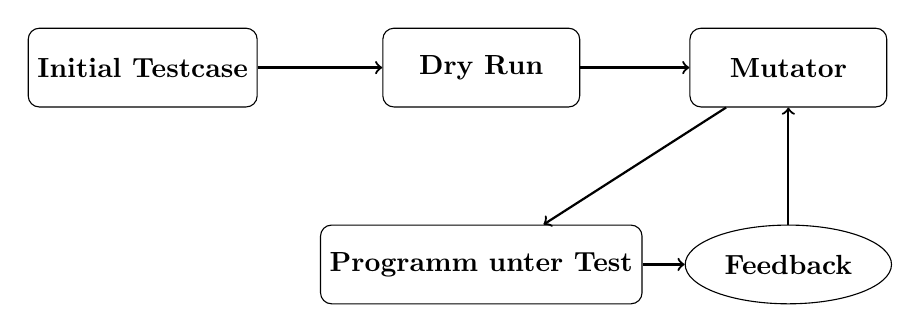
\begin{tikzpicture}[node distance=2.5cm]
        \node[draw, rectangle, rounded corners, minimum height=1cm, minimum width=2.5cm] (testcase) {\textbf{Initial Testcase}};
        \node[draw, rectangle, rounded corners, minimum height=1cm, minimum width=2.5cm, right of=testcase, xshift=1.8cm] (dryrun) {\textbf{Dry Run}};
        \node[draw, rectangle, rounded corners, minimum height=1cm, minimum width=2.5cm, right of=dryrun, xshift=1.4cm] (mutator) {\textbf{Mutator}};
        \node[draw, rectangle, rounded corners, minimum height=1cm, minimum width=2.5cm, below of=dryrun] (program) {\textbf{Programm unter Test}};
        \node[draw, ellipse, minimum height=1cm, minimum width=2.2cm, right of=program, xshift=1.4cm] (feedback) {\textbf{Feedback}};

        \draw[->, thick] (testcase) -- (dryrun);
        \draw[->, thick] (dryrun) -- (mutator);
        \draw[->, thick] (mutator) -- (program);
        \draw[->, thick] (program) -- (feedback);
        \draw[->, thick] (feedback) -- (mutator);
    \end{tikzpicture}
\end{frame}
\begin{frame}{Wie Funktionert Fuzzing?}
    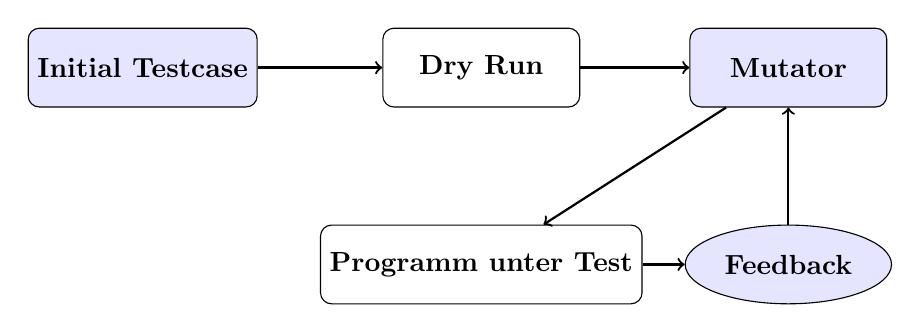
\begin{tikzpicture}[node distance=2.5cm]
        \node[draw, rectangle, rounded corners, minimum height=1cm, minimum width=2.5cm, fill=blue!10] (testcase) {\textbf{Initial Testcase}};
        \node[draw, rectangle, rounded corners, minimum height=1cm, minimum width=2.5cm, right of=testcase, xshift=1.8cm] (dryrun) {\textbf{Dry Run}};
        \node[draw, rectangle, rounded corners, minimum height=1cm, minimum width=2.5cm, right of=dryrun, xshift=1.4cm, fill=blue!10] (mutator) {\textbf{Mutator}};
        \node[draw, rectangle, rounded corners, minimum height=1cm, minimum width=2.5cm, below of=dryrun] (program) {\textbf{Programm unter Test}};
        \node[draw, ellipse, minimum height=1cm, minimum width=2.2cm, right of=program, xshift=1.4cm, fill=blue!10] (feedback) {\textbf{Feedback}};

        \draw[->, thick] (testcase) -- (dryrun);
        \draw[->, thick] (dryrun) -- (mutator);
        \draw[->, thick] (mutator) -- (program);
        \draw[->, thick] (program) -- (feedback);
        \draw[->, thick] (feedback) -- (mutator);
    \end{tikzpicture}
\end{frame}
\section{Demo}\label{sec:demo2}
\begin{frame}{Herausforderung von Fuzzing}
    \begin{itemize}
        \item Lückenhafte Codeabdeckung
        \item Unzureichende Testfälle
        \item Verstehen von komplexen Codepfaden
        \item Nichtdeterministische Programme und zustandsabhängige Systeme
    \end{itemize}
\end{frame}
    %! Author = chaorn
%! Date = 11.12.24

\section{Das innere eines Fuzzers}\label{sec:das-innere-eines-fuzzers}
\begin{frame}{Was steckt in einem Fuzzer?}
    \begin{itemize}
        \item \alert{Corpus}
        \item Input Generator
        \item Mutator
        \item Laufzeitumgebung für das zu untersuchende System
        \item Monitoring
        \item \alert{Strategie}
    \end{itemize}
\end{frame}
\begin{frame}{Corpus}
    \begin{itemize}
        \item Sammlung von Testcases (initial händisch)
        \item Wird durch den Fuzzer verwaltet
        \item Wird durch den Mutator verändert
        \item Wird durch den Input Generator erweitert/verkleinert
    \end{itemize}
\end{frame}
\begin{frame}{Input Generator}
    Am Beispiel von AFL(American Fuzzy Lop):
    \begin{itemize}
        \item Generiert Testcases anhand des Corpus
        \item Verwendet bevorzugt Testcases, die zu einer höheren Codeabdeckung führen
    \end{itemize}
\end{frame}
\begin{frame}{Mutator}
    \begin{itemize}
        \item Verändert Testcases
        \item Mutationsstrategien:
              \begin{itemize}
                  \item Bitflips
                  \item Byteflips
                  \item Arithmetische Operationen
                  \item Block Operationen
                  \item Splicing
                  \item \ldots
              \end{itemize}
    \end{itemize}
\end{frame}
\begin{frame}{Laufzeitumgebung}
    \begin{itemize}
        \item Stellt das zu untersuchende System bereit
        \item Am weitesten Verbreitet: QEMU
        \item Kann auf verschiedene Arten konfiguriert werden
        \item Sorgt für Isolation des zu untersuchenden Systems
        \item Ermöglicht Cross-Plattform Kompatibilität (z.B. Fuzzing von ARM auf x86 Host)
    \end{itemize}
\end{frame}
\begin{frame}{Einschub: Low Level Fundamentals}
    \begin{itemize}
        \item Was ist ein Basic Block?
        \item Was ist Codeabdeckung?
        \item Was ist ein Codepfad?
    \end{itemize}
\end{frame}
\begin{frame}{Low Level Fundamentals}
    \textbf{Basic Block:} Ein Basic Block ist eine Sequenz von Anweisungen, die von einem Punkt im Programmfluss bis zu einem Sprungbefehl führen.\break
    \textbf{Codeabdeckung:} Codeabdeckung ist ein Maß dafür, wie viele Basic Blocks eines Programms durch Testcases erreicht werden.\break
    \textbf{Codepfad:} Ein Codepfad ist eine Sequenz von Basic Blocks, die durch einen Testcase erreicht werden.
\end{frame}
\begin{frame}{Low Level Fundamentals}
    \begin{figure}[H]
        \centering
        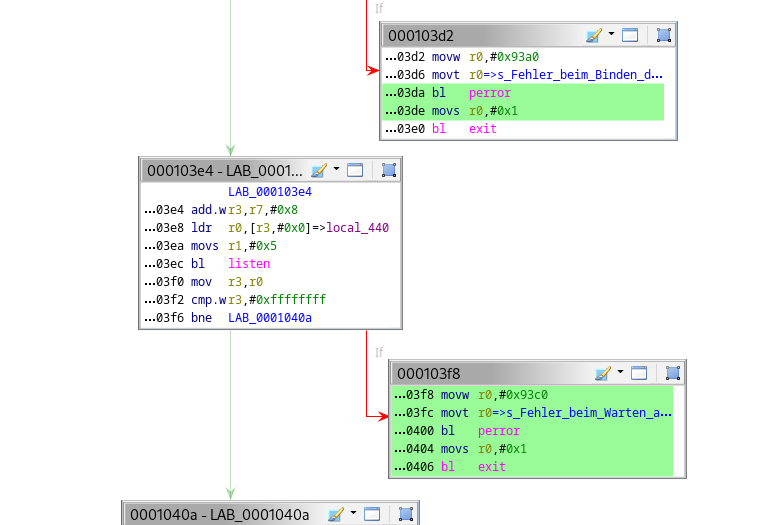
\includegraphics[width=\textwidth]{res/basic_block_example}
        \caption[Basic Blocks am Beispiel eines selbst implementierten TCP Server]{Basic Blocks am Beispiel eines selbst implementierten TCP Server}
        \label{fig:basic-blocks}
    \end{figure}
\end{frame}
\begin{frame}{Low Level Fundamentals}
    \begin{figure}[H]
        \centering
        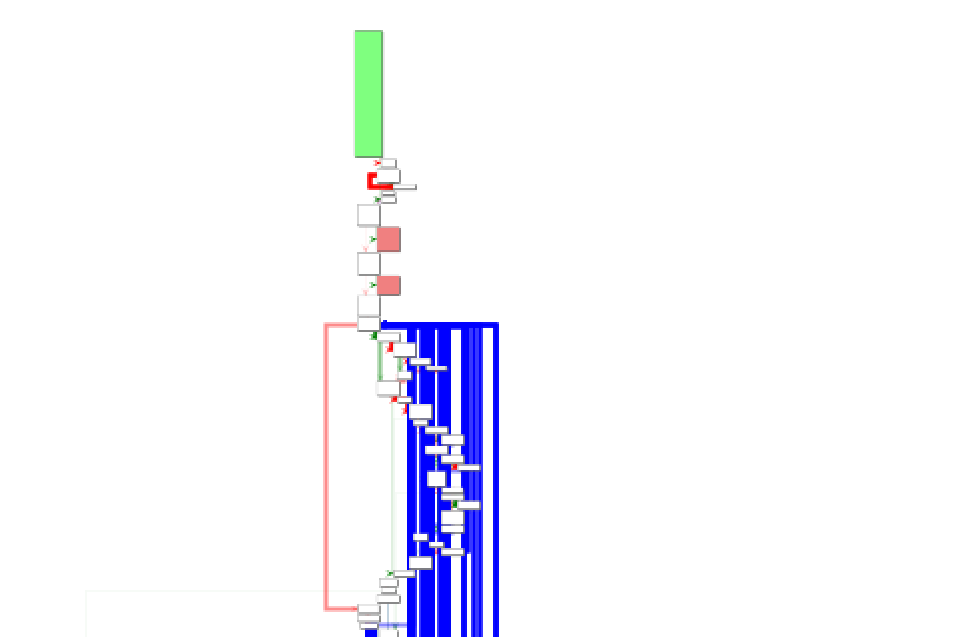
\includegraphics[width=\textwidth]{res/call_graph_ssh}
        \caption[Code Blocks am Beispiel des ssh Binary]{Code Blocks am Beispiel des ssh Binary}
        \label{fig:code-coverage}
    \end{figure}
\end{frame}
\begin{frame}{Monitoring}
    \begin{itemize}
        \item Überwacht das zu untersuchende System
        \begin{itemize}
            \item Codeabdeckung
            \item Laufzeit
            \item Speicherverbrauch
            \item Crashes
            \item \ldots
        \end{itemize}
        \item Oft auf Basis von Instrumentierung
        \item Kann größtenteils über die Laufzeitumgebung realisiert werden
    \end{itemize}
\end{frame}
\begin{frame}{Strategie}
    \begin{itemize}
        \item Steuert den Ablauf des Fuzzers
        \item Bestimmt, welcher Testcase wann verwendet wird
        \begin{itemize}
            \item Codeabdeckung (AFL) = Wie viele (neue) Basic Blocks werden durch den Testcase traversiert?
            \item Zielgerichtet (Dowser) = Spezifische Codepfade, die durch den Testcase erreicht werden sollen
        \end{itemize}
    \end{itemize}
\end{frame}
\section{Techniken des Fuzzings}\label{sec:techniken-des-fuzzings}
\begin{frame}{Techniken des Fuzzings}
    \begin{itemize}
        \item Mutation (AFL)
        \item Generation (boofuzz)
        \item \alert{Machine Learning \& KI} (Pulsar)
    \end{itemize}
\end{frame}

    %! Author = chaorn
%! Date = 11.12.24

\section{Machine Learning und Fuzzing}\label{sec:machine-learning-und-fuzzing}
\begin{frame}{Machine Learning und Fuzzing}
    Wieso Machine Learning und Fuzzing?
    \begin{itemize}
        \item Machine Learning kann interessante Eingaben vorhersagen
        \item Komplexe Strukturen von Eingaben können erkannt werden
        \item Verbessertes Verständnis von Code(-fehl-)verhalten
    \end{itemize}
\end{frame}
\begin{frame}{Begin von Machine Learning und Fuzzing}
    \begin{figure}[H]
        \centering
        
\includegraphics[width=\textwidth]{res/pulsar}
        \caption[Pioniere des Fuzzing mit Machine Learning]{
            Veröffentlichung des ersten Fuzzers mit statistischen Modellen~\cite{thuraisingham_pulsar_2015}
        }
        \label{fig:ml_fuzzing}
    \end{figure}
\end{frame}
\begin{frame}{Pulsar}
    \begin{itemize}
        \item Erster Fuzzer mit \enquote{Machine Learning}
        \item Verwendung von Markov-Modellen
        \item Erkennt und simuliert Zustände
        \item Erkennt und simuliert Nachrichten
        \item Kann sowohl ein Protokoll simulieren, als auch das tatsächliche Protokoll fuzzen
    \end{itemize}
\end{frame}
\section{Demo}\label{sec:demo}
\begin{itemize}
    \item Role of Convolutional Neural Networks in fuzzing:
    \begin{itemize}
        \item Analyzing code structure and coverage patterns.
        \item Input prioritization using learned models.
    \end{itemize}
        \item Feature extraction from execution traces and call graphs.
        \item Example application: Predicting program branches that require exploration.
\end{itemize}

\begin{itemize}
    \item Challenges in using ML for fuzzing:
    \begin{itemize}
        \item High computational requirements.
        \item Training data scarcity for certain domains.
    \end{itemize}
    \item Future possibilities:
    \begin{itemize}
        \item Reinforcement learning for fuzzing optimization.
        \item Transfer learning to adapt fuzzers to new domains.
    \end{itemize}
\end{itemize}

    \printbibliography[title={Quellen}]
\end{document}